% -*- coding: utf-8; mode: latex; -*-

% +++
% latex = "lualatex"
% +++

%
% FIT2023 向け LaTeX クラスファイル
% https://github.com/trueroad/FITpaper-class
%
% サンプルファイル
%
% Copyright (C) 2018, 2019, 2022, 2023 Masamichi Hosoda.
% All rights reserved.
%

\documentclass{FITpaper}

% 図の貼り込み用
\usepackage{graphicx}

% 最終ページで両カラムの下端を揃える
%\usepackage[balance]{nidanfloat}
\usepackage{flushend}
\def\BibTeX{{\rm B\kern-.05em{\sc i\kern-.025em b}\kern-.08em
    T\kern-.1667em\lower.7ex\hbox{E}\kern-.125emX}}
% 和文タイトル
\jtitle{ブラウザ上でユーザが編集可能な言語パターンマッチシステムの構築 }

% 欧文タイトル
\etitle{Building a user-editable language pattern matching system in the browser}

% 著者数:著者の数だけ c を書く
\authors{cc}

% 和文著者名:著者名間に & を書く
% 所属番号を \affmark でつける
\jauthors{%
  桂 辰弥\affmark{1} &
  竹内 孔一\affmark{1}
}

% 欧文著者名:著者名間に & を書く
\eauthors{%
  Tatsuya Katsura &
  Koichi Takeuchi
}

% 所属
% \affmark でつけた番号毎に指定
\afftext{1}{岡山大学}


\begin{document}

\maketitle

\section{はじめに}
テキスト中の特定のフレーズや表現を見つけることは,言語および教育分野において必要となることがある.テキストデータから特定のキーワードやフレーズの出現位置や文脈を抽出するためのプログラムとしてコンコーダンサがある.コンコーダンサは語学学習において特定のフレーズや表現の使用例を実際の文脈で把握することで,語彙や文法の理解、単語の使用法や文脈の把握に役立ち,学習者の語彙や表現力の向上に役立つ.
パターンマッチングはテキストの表層で検索を行う正規表現とは異なり,情報を抽出したい文を対象に予め関係する文や文の一部に対応する文構造のパターンを用意し,そのパターンに合致する結果を取得するものである.
有名なコンコーダンサの例として,Sketch Engineがある.Sketch Engine\footnote{https://www.sketchengine.eu/},はクエリ言語としてCQL(Corpus Query Language)\footnote{https://www.sketchengine.eu/documentation/corpus-querying/}が使用されており,コーパス内で正規表現や演算子を組み合わせることでパターンマッチを行うことができる.
しかしSketch Engineは,コーパスベースの言語分析や統計的な情報抽出が主な役割であるため,
テキスト中から依存関係解析を持つ表現を抽出する際には前処理が必要となる.

ユーザ自らがこれらを考慮してテキスト中の特定フレーズや表現を抽出するようなシステムを構築することは容易ではない.そこで本研究では解析モジュールで解析した結果をユーザ自身が求める表現をあらかじめ用意された検索ブロックで組み合わせてシステムに投入し,事例を検索できるシステムの開発を行っている.先行研究においてWEBアプリケーションとしてJavaScriptとPythonを利用した基本システムを構築したが,
システムの本格利用にはいくつかの課題が残されている.そこで本報告では検索エンジンの中心部分であるPrologデータベースの実装の改良,および,大規模なテキストが扱えるためにデータベースをシステムに導入したので、この改良について報告する.


\section{提案するパターンマッチシステムの概要}
本章では開発したパターンマッチシステムを構築する環境と実際のシステムの処理の流れについて述べる.
また先行研究との大きな変更点であるPrologデータベースの実装の改良,および,大規模なテキストが扱えるためにデータベースをシステムに導入についても触れている.

\subsection{提案するパターンマッチシステムの構成}

\begin{figure}[htbp]
  \centering
  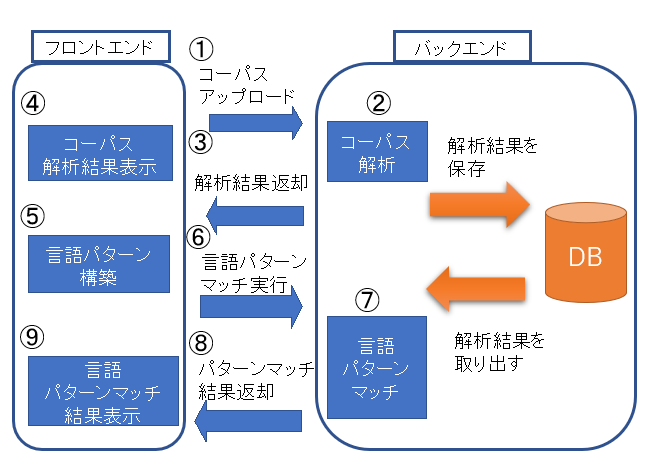
\includegraphics[scale=0.4]{fig/system_fig.png}
  \caption{システムの構成図}
  \label{fig:sys}
\end{figure}

本システムは図\ref{fig:sys}のようにユーザが視覚的に操作を行うフロントエンドシステムとユーザが要求したテキストの処理バックエンドシステムに切り分けて構成している.

フロントエンドシステムはJavascriptのライブラリであるReact.jsで構成されており
主な機能としてはテキストファイルのアップロード,検索する言語パターンの構築,解析結果の表示,検索結果の表示などがある.

バックエンドシステムはPythonのWebフレームワークであるDjangoとデータベースシステムであるElasticsearchで構成されており,
主な機能としてはテキストファイルの解析,ユーザが構築した検索クエリの言語パターンマッチ実行などがある.



詳しい処理の流れについては以降の節で述べる.

\subsection{バックエンドの処理の流れについて}
バックエンドの処理の流れとしてテキスト解析,言語パターンマッチ実行の処理についてそれぞれ説明する.

\begin{figure}[htbp]
  \centering
  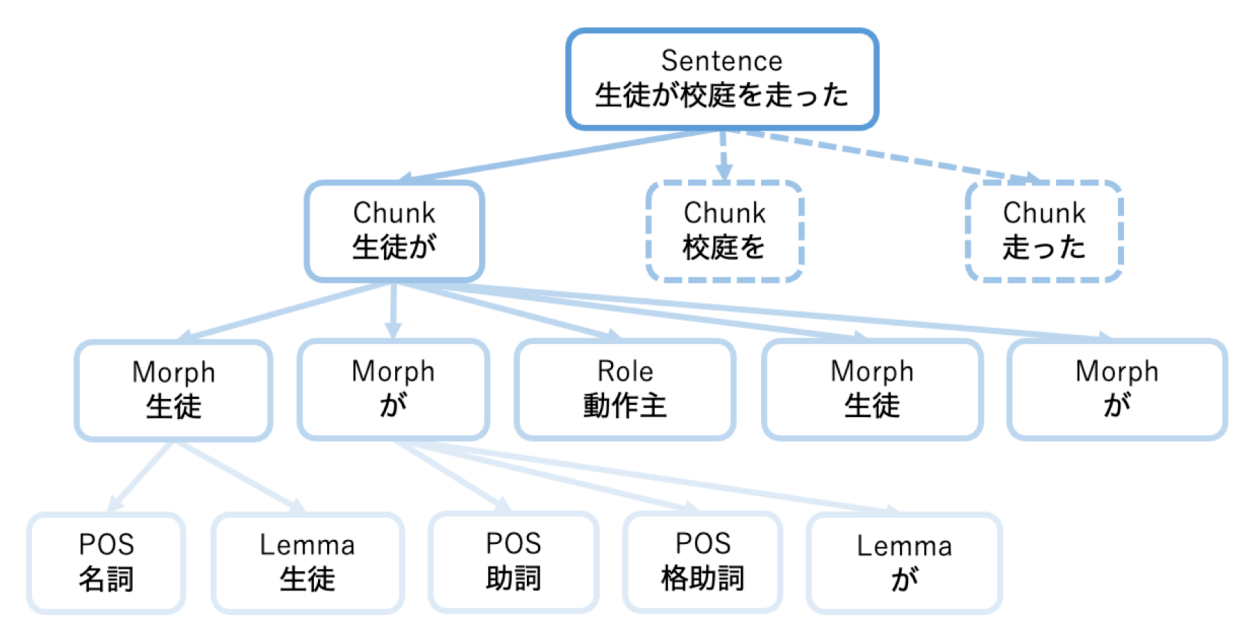
\includegraphics[scale=0.4]{fig/tree.eps}
  \caption{文を解析した木構造の例}
  \label{fig:tree}
\end{figure}
\begin{table}[htbp]
  \caption{Prologの述語一覧}
  {\footnotesize
  \begin{center}
    \begin{tabular}{|l|l|l|l|}\hline
      述語                    &第1引数     &  第2引数   & 第3引数               \\
      \hline 

      chunk(\_, 0,\_)       &文番号    &  0固定& 文節 ID                   \\
      morph(\_, \_, \_)     &文番号 & 文節 ID& 形態素 ID                \\
      main(\_, \_, \_)      &文番号   &文節 ID & 主形態素 \\
      part(\_, \_, \_)      &文番号   &文節 ID& 副形態素\\
      role(\_, \_, \_)      &文番号   &文節 ID& 意味役割  \\
      semantic(\_, \_, \_)   &文番号  &文節 ID & 概念\\
      surf(\_, \_, \_)        &文番号  &ノード ID& 表層\\               
      surfBF(\_, \_, \_)      &文番号 &形態素 ID& 基本形        \\
      sloc(\_, \_, \_)  &文番号&文節/形態素 ID & 文中出現位置\\
      pos(\_, \_, \_)    &文番号      &形態素 ID& 品詞\\                                        
      dep(\_, \_, \_)     &文番号   &文節 ID & 係り受け文節 ID\\
        \hline
    \end{tabular}
  
    \label{tbl:predicates}
  \end{center}
  }
\end{table}

テキスト解析の処理はユーザがテキストファイルのアップロードを行うことで実行される.送られたテキストファイルの文にASA{}を用いて形態素解析,係り受け解析,項構造解析を適応させる.解析した結果の文の木構造を図\ref{fig:tree}に示す.
その後Prolog述語に変換を行い,データベースに保存する.変換するProlog述語は以下の表\ref{tbl:predicates}のように定義している.%図\ref{fig:prolog}のように変換される.

ASAで解析したデータがJSON形式であるため,Elasticsearchをデータベースとして活用することで,
JSON形式の大規模な解析データの柔軟な取り扱いや高速な検索,リアルタイムな更新,スケーラビリティ,高度な分析など,データベースとしての利点を最大限に生かすことができる.



言語パターンマッチの処理はフロントエンドからユーザが構築した検索パターンが送られるとデータベースから各文に対応するPrologを取得し,Prologパターンマッチが実行される.
パターンマッチを実行するProlog処理系としてSWI-Prologのpythonモジュールであるpyswipを使用している.
Prolog処理系として採用したSWI-PrologはCで書かれた高機能のProlog処理系であり,
SWI-Prologの強力な論理プログラミング機能とPythonのデータ処理能力を組み合わせることで,高速でより拡張性の高い環境が提供される.

また先行研究のシステムとのバックエンドの大きな改良点としては
バックエンド側でデータベースに保存する際に,以前は全文の解析データを1つのデータとして保存していたが,このために保存できる解析データに制限がかかってしまっていたため,
1文ごとに対応した解析データを保存するように改良を行った.
またデータベースの取得を1文ずつPrologデータベースの処理を行い,マッチ解の生成を行うように改良した.





%\begin{figure}[htbp]
 % \centering
  %\includegraphics[scale=0.5]{fig/prolog_data.png}
  %\caption{変換されたprolog}
  %\label{fig:prolog}
%\end{figure}


\subsection{フロントエンドの表示機能について}
次にフロントエンドでの解析結果,検索クエリとなる言語パターンの構築,検索結果の表示について説明する.

\begin{figure}[htbp]
  \centering
  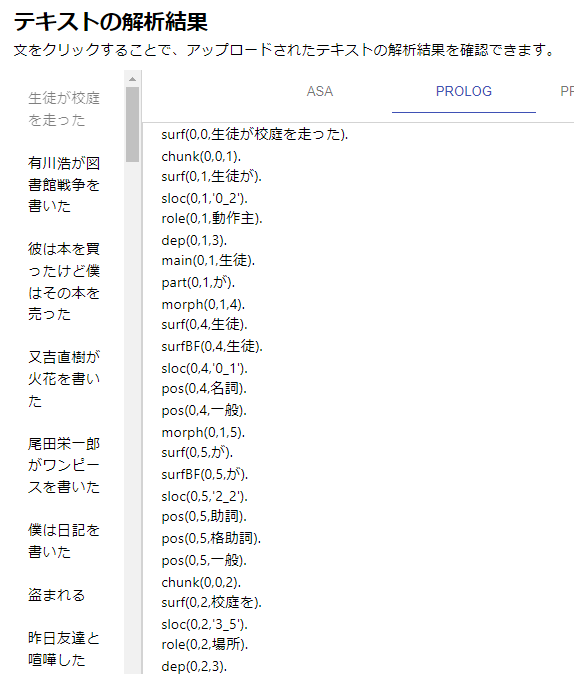
\includegraphics[scale=0.4]{fig/convert_result_prolog.png}
  \caption{解析結果の例}
  \label{fig:show_prolog}
\end{figure}



\begin{figure}[htbp]
  \centering
  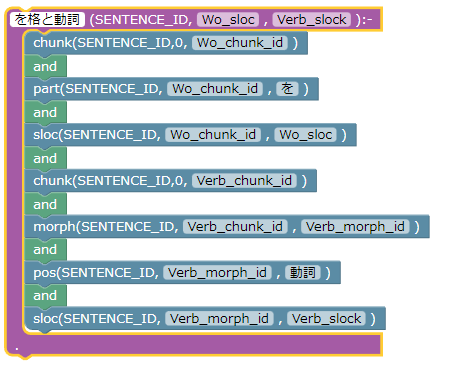
\includegraphics[scale=0.6]{fig/wo.png}
  \caption{「ヲ格と動詞」の検索パターン}
  \label{fig:wo_block}
\end{figure}

\begin{figure}[htbp]
  \centering
  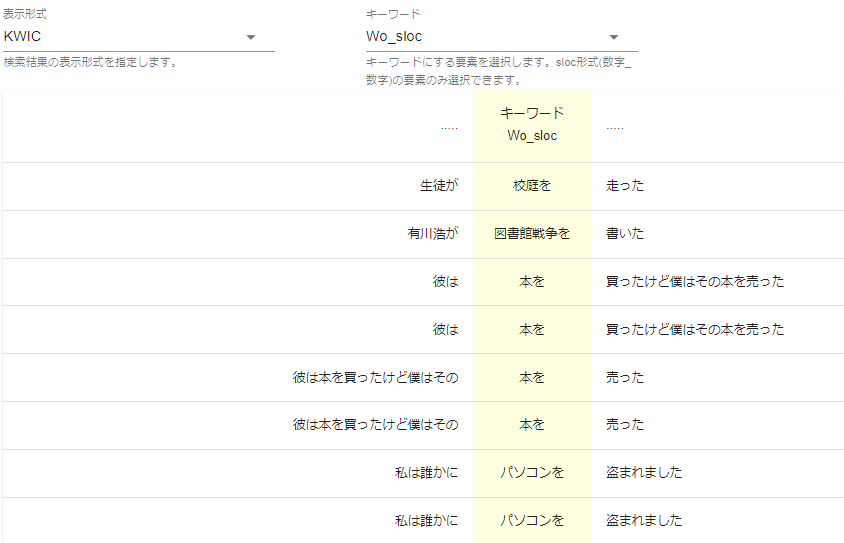
\includegraphics[scale=0.4]{fig/KWIC_result.png}
  \caption{KWIC表示}
  \label{fig:KWIC}
\end{figure}
\begin{figure}[htbp]
  \centering
  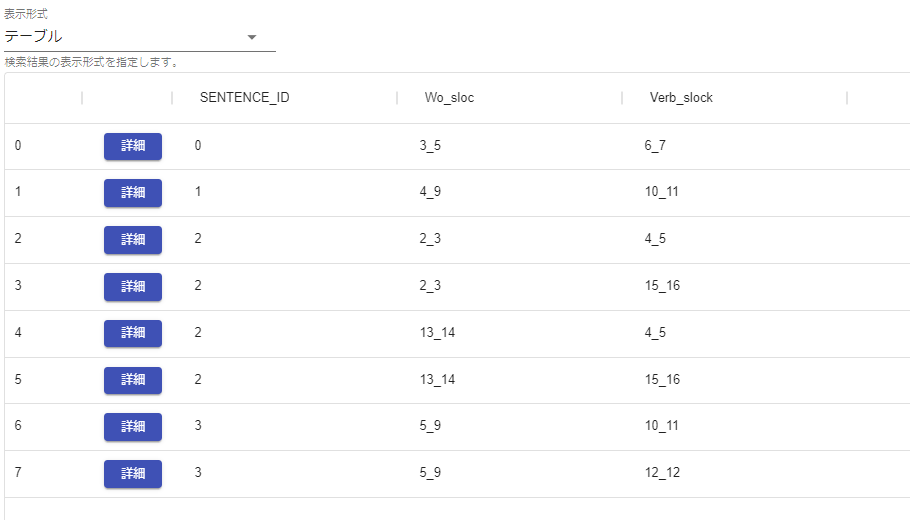
\includegraphics[scale=0.4]{fig/table_result.png}
  \caption{テーブル表示}
  \label{fig:table}
\end{figure}
\begin{figure}[htbp]
  \centering
  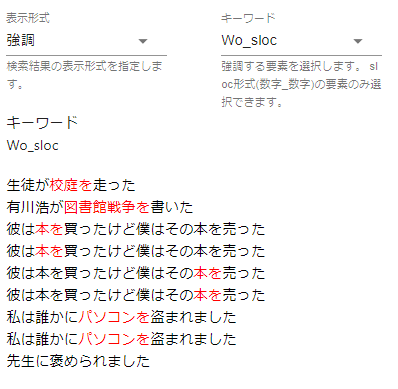
\includegraphics[scale=0.4]{fig/acsent_result.png}
  \caption{強調表示}
  \label{fig:acsent}
\end{figure}

フロントエンドはテキスト解析の処理終了後,解析結果をデータベースから取得して表示できる.以下の図\ref{fig:show_prolog}は解析結果の表示例である.

先行研究のシステムとの変更点として,
1文ごとに対応した解析データを保存するようにデータベースに保存する変更を行ったため,解析データの表示の際にはクリックした文の解析データがそれぞれ取得するように改良を行った.

言語パターンを構築する際にはBlocklyを用いて生成できる.
前節で示したProlog述語のブロックをユーザが自ら組み合わせることで,複雑な検索クエリを構築することができる.
図\ref{fig:wo_block}はその例である.検索実行後,バックエンドから検索結果を受信し,結果の表示の際にはKWIC,テーブル,強調の3つの表示形式を用いることができる.
以下の図\ref{fig:KWIC},\ref{fig:table},\ref{fig:acsent}は図\ref{fig:wo_block}の検索結果の表示例である.
引数\textit{Wo\_Slock},\textit{Verb\_Slock}は文中での出現位置を示しており,検索パターンの引数に\textit{\_slock}を含む場合と表示形式で強調する要素を選択できるようになる.
図\ref{fig:KWIC}は「ヲ格」,図\ref{fig:acsent}は「動詞」の要素を強調して表示し,視覚的にわかりやすくなっている.




\section{動作評価実験}
システムの動作評価実験を行い,パターンマッチシステムの処理性能の向上の確認を行う.

\subsection{実験内容}
\begin{table}[htbp]
  \centering
    \caption{ファイルサイズ(バイト)}
    \label{fig:tex}
    \begin{tabular}{|l||r|}  
      \hline
      文の数 & ファイルサイズ\\ \hline \hline
      1 & 46\\\hline
      10 & 440 \\\hline
      100 & 5,342\\ \hline
      1000 & 53,248 \\\hline
      5000 &  262,199 \\\hline
      10000 &  524,399\\ \hline
    \end{tabular}
  \end{table}

図\ref{fig:convert_time}に示すテキストファイルを用意し,
テキスト解析とパターンマッチを行い,これらの処理時間を先行研究のシステムと提案するパターンマッチシステムでそれぞれ計測した.
具体的にはフロントエンドからバックエンドに送信し,バックエンドからデータが返ってくるまでを処理時間として計測する.
これらの処理時間はChromeのデベロッパーツールを用いて計測を行う.
検索クエリは図\ref{fig:wo_block}の「ヲ格と動詞」の言語パターンを用いる.


\subsection{実験結果}

\begin{table}[htbp]
  \centering
    \caption{テキスト解析の処理時間(秒)}
    \label{fig:convert_time}
    \begin{tabular}{|r||r|r|}  
      \hline
      文の数 &先行研究のシステム& 提案するシステム \\\hline \hline
      1 & 0.140&0.144\\\hline
      10 & 0.442&0.403 \\\hline
      100 & 1.47 &3.56\\ \hline
      1000 & 28.9&36.4 \\\hline
      5000 &  144&192\\\hline
      10000 &  計測不能&768\\ \hline
    \end{tabular}
  \end{table}
\begin{table}[htbp]
  \centering
    \caption{パターンマッチの処理時間(秒)}
    \label{fig:matching_time}
    \begin{tabular}{|l||r|r|}  
      \hline
      文の数 & 先行研究のシステム& 提案するシステム\\ \hline \hline
      1 & 0.110&0.242\\\hline
      10 & 0.531 &0.495\\\hline
      100 & 4.41&1.65\\ \hline
      1000 & 58 &30.9 \\\hline
      5000 & 290 &78.4\\\hline
      10000 & 計測不能 &160\\ \hline
    \end{tabular}
  \end{table}


  パターンマッチの動作評価実験の結果をそれぞれ表\ref{fig:convert_time},\ref{fig:matching_time} に示す.
  テキスト解析,パターンマッチ実行はともに文の数が増えるにつれ,処理時間も増加していることが読み取れる.
  テキスト解析の処理時間は先行研究のシステムに比べ,少し遅くなったが,
  先行研究のシステムは10000文を解析できなかったが,提案するパターンマッチシステムは解析可能となり,パターンマッチ実行処理も確認できた.
  これらの結果からシステムの処理性能の向上が確認できた.
  
\section{考察}
  この章では実験の考察から,今後の改良に向けた案を提案する.
  テキスト解析の処理時間は先行研究のシステムに比べ,少し遅くなったが,これはデータベースを1文ごとに対応した解析データを保存するように改良を行ったためであり,
  10000文を解析を行った際には10000個の解析データを保存する必要があるため,バックエンドでのDjangoとデータベースシステムとのやりとりの時間が増加してしたためである.



  
  今回の実装では1文ずつprologデータベースに追加し,パターンマッチを生成したが,
  これは全文のprologデータベースの処理を行うファイルの生成に時間がかかるため,1文ずつ生成するように変更した.
  このことにより,処理速度が向上したが,これは全文のprologデータを記載した大規模なファイルを生成する必要があったためである.
  例えば10000文のパターンマッチを行う際には10000回処理を行うprologファイルの生成を行う必要があるため,バックエンドシステムへの負荷が大きいため,
  ファイル生成を行わずにパターンマッチを実行する実装方法を検討する必要がある.
  Elasticsearchは、1度に取得することができるドキュメントの最大件数は、デフォルトでは10,000件であるためであり,
  10000文以上のテキストファイルの解析は現状のシステムでは不可能である.
  また提案するパターンマッチシステムは10000文を解析可能となったが,さらに解析後のブラウザの挙動がかなり重くなっており,
  ユーザが利用可能とは言い難い.
  今後さらに処理性能の向上させるには,パフォーマンスの問題やネットワークの制約などに留意して実装する必要となる.
  

\section{まとめ}
Prolog 処理系の問題や解析対象のテキストの文数の上限や動作速度の問題,そ
れらの問題についての改善案を提示し,改善案に基づいてシステムを構築した.具体的には
Prolog 処理系を Python 疑似コードで作成していた prologpy から Prologpy 処理系である
SWI-Prolog に変更した.テキストの保存方法が制限があるブラウザのメモリからデータ
ベースサーバである Elasticsearch に変更した.テキストの保存方法を制限があるブラウザ
のメモリからデータベースサーバである Elasticsearch に変更し,テキストの保存方法を制
限があるブラウザのメモリからデータベースサーバである Elasticsearch に変更し,関連す
る処理をすべて変更した.実装機能の評価実験の結果,5000 程度であれば問題なく動作す
ることを示した.今後の課題としては,より大規模なテキストの解析およびパターンマッチ
について動作可能になるようデータベースの改良を行う.また,パターンマッチ時のユー
ザの待ち時間の間に,ユーザが他の機能を操作可能にすることを実現したい.さらに,新た
な機能案として正規表現マッチや解析する言語の切り替えを挙げ,Web アプリケーション
としてより実用可能なパターンマッチシステムを目指す.
\acknowledgment{%
  謝辞の文章を\texttt{\textbackslash acknowledgment}で指定します。
  使わなければ謝辞は出力されません。
}

%\bibliographystyle{unsrt}

%\bibliography{all,my-results}


\end{document}